\documentclass[12pt,a4paper]{report}
\usepackage[utf8]{inputenc}
\usepackage{amsmath}
\usepackage{amsfonts}
\usepackage{amssymb}
\usepackage{amsthm}
\usepackage{hyperref}
\usepackage{mathrsfs}

\usepackage{multicol}
\usepackage{fancyhdr}
\usepackage[inline]{enumitem}
\usepackage{tikz}
\usepackage{tikz-cd}
\usetikzlibrary{calc}
\usetikzlibrary{shapes.geometric}
\usetikzlibrary{positioning}
\usepackage[margin=0.5in]{geometry}
\usepackage{xcolor}

\hypersetup{
    colorlinks=true,
    linkcolor=blue,
    filecolor=magenta,      
    urlcolor=cyan,
    pdftitle={Tensors},
    pdfpagemode=FullScreen,
    }

%\urlstyle{same}

\newcommand{\CLASSNAME}{Math XXXX -- Independent Study: Manifolds}
\newcommand{\STUDENTNAME}{Paul Carmody}
\newcommand{\ASSIGNMENT}{\textit{Basic Category Theory -- Tom Leinster}}
\newcommand{\DUEDATE}{August, 2025}
\newcommand{\PROFESSOR}{Professor Berchenko-Kogan}
\newcommand{\SEMESTER}{Summer 2025}
\newcommand{\SCHEDULE}{TBD}
\newcommand{\ROOM}{Edinburgh}

\newcommand{\MMN}{M_{m\times n}}
\newcommand{\FF}{\mathcal{F}}

\pagestyle{fancy}
\fancyhf{}
\chead{ \fancyplain{}{\CLASSNAME} }
%\chead{ \fancyplain{}{\STUDENTNAME} }
\rhead{\thepage}
\newcommand{\LET}{\text{Let }}
%\newcommand{\IF}{\text{if }}
\newcommand{\AND}{\text{ and }}
\newcommand{\OR}{\text{ or }}
\newcommand{\FORSOME}{\text{ for some }}
\newcommand{\FORALL}{\text{ for all }}
\newcommand{\WHERE}{\text{ where }}
\newcommand{\WTS}{\text{ WTS }}
\newcommand{\WLOG}{\text{ WLOG }}
\newcommand{\BS}{\backslash}
\newcommand{\DEFINE}[1]{\textbf{\emph{#1}}}
\newcommand{\IF}{$(\Rightarrow)$}
\newcommand{\ONLYIF}{$(\Leftarrow)$}
\newcommand{\ITH}{\textsuperscript{th} }
\newcommand{\FST}{\textsuperscript{st} }
\newcommand{\SND}{\textsuperscript{nd} }
\newcommand{\TRD}{\textsuperscript{rd} }
\newcommand{\INV}{\textsuperscript{-1} }

\newcommand{\XXX}{\mathfrak{X}}
\newcommand{\MMM}{\mathfrak{M}}
%\newcommand{\????}{\textfrak{A}}
%\newcommand{\????}{\textgoth{A}}
%\newcommand{\????}{\textswab{A}}

\DeclareMathOperator{\DER}{Der}
\DeclareMathOperator{\SGN}{sgn}

%%%%%%%
% derivatives
%%%%%%%

\newcommand{\PART}[2]{\frac{\partial #1}{\partial #2}}
\newcommand{\SPART}[2]{\frac{\partial^2 #1}{\partial #2^2}}
\newcommand{\DERIV}[2]{\frac{d #1}{d #2}}
\newcommand{\LAPLACIAN}[1]{\frac{\partial^2 #1}{\partial x^2} + \frac{\partial^2 #1}{\partial y^2}}

%%%%%%%
% sum, product, union, intersections
%%%%%%%

\newcommand{\SUM}[2]{\underset{#1}{\overset{#2}{\sum}}}
\newcommand{\PROD}[2]{\underset{#1}{\overset{#2}{\prod}}}
\newcommand{\UNION}[2]{\underset{#1}{\overset{#2}{\bigcup}}}
\newcommand{\INTERSECT}[2]{\underset{#1}{\overset{#2}{\bigcap}}}
\newcommand{\FSUM}{\SUM{n=-\infty}{\infty}}
       

%%%%%%%
% supremum and infimum
%%%%%%%

\newcommand{\SUP}[1]{\underset{#1}\sup \,}
\newcommand{\INF}[1]{\underset{#1}\inf \,}
\newcommand{\MAX}[1]{\underset{#1}\max \,}
\newcommand{\MIN}[1]{\underset{#1}\min \,}

%%%%%%%
% infinite sums, limits
%%%%%%%

\newcommand{\SUMK}{\SUM{k=1}{\infty}}
\newcommand{\SUMN}{\SUM{n=1}{\infty}}
\newcommand{\SUMKZ}{\SUM{k=0}{\infty}}
\newcommand{\LIM}[1]{\underset{#1}\lim\,}
\newcommand{\IWOB}[1]{\LIM{#1 \to \infty}}
\newcommand{\LIMK}{\IWOB{k}}
\newcommand{\LIMN}{\IWOB{n}}
\newcommand{\LIMX}{\IWOB{x}}
\newcommand{\NIWOB}{\LIM{n \to \infty}}
\newcommand{\LIMSUPK}{\underset{k\to\infty}\limsup \,}
\newcommand{\LIMSUPN}{\underset{n\to\infty}\limsup \,}
\newcommand{\LIMINFK}{\underset{k\to\infty}\liminf \,}
\newcommand{\LIMINFN}{\underset{n\to\infty}\liminf \,}
\newcommand{\ROOTRULE}[1]{\LIMSUPK \BARS{#1}^{1/k}}

\newcommand{\CUPK}{\bigcup_{k=1}^{\infty}}
\newcommand{\CAPK}{\bigcap_{k=1}^{\infty}}
\newcommand{\CUPN}{\bigcup_{n=1}^{\infty}}
\newcommand{\CAPN}{\bigcap_{n=1}^{\infty}}

%%%%%%%
% number systems (real, rational, etc.)
%%%%%%%

\newcommand{\REALS}{\mathbb{R}}
\newcommand{\RATIONALS}{\mathbb{Q}}
\newcommand{\IRRATIONALS}{\REALS \backslash \RATIONALS}
\newcommand{\INTEGERS}{\mathbb{Z}}
\newcommand{\NUMBERS}{\mathbb{N}}
\newcommand{\COMPLEX}{\mathbb{C}}
\newcommand{\DISC}{\mathbb{D}}
\newcommand{\HPLANE}{\mathbb{H}}

\newcommand{\R}{\mathbb{R}}
\newcommand{\Q}{\mathbb{Q}}
\newcommand{\Z}{\mathbb{Z}}
\newcommand{\N}{\mathbb{N}}
\newcommand{\C}{\mathbb{C}}
\newcommand{\T}{\mathbb{T}}
\newcommand{\COUNTABLE}{\aleph_0}
\newcommand{\UNCOUNTABLE}{\aleph_1}


%%%%%%%
% Arithmetic/Algebraic operators
%%%%%%%


\DeclareMathOperator{\MOD}{mod}
%\newcommand{\MOD}[1]{\mod #1}
\newcommand{\BAR}[1]{\overline{#1}}
\newcommand{\LCM}{\text{ lcm}}
\newcommand{\ZMOD}[1]{\Z/#1\Z}
\DeclareMathOperator{\VAR}{Var}
%%%%%%%
% complex operators
%%%%%%%

\DeclareMathOperator{\RR}{Re}
%\newcommand{\RE}{\text{Re}}
\DeclareMathOperator{\IM}{Im}
%\newcommand{\IM}{\text{Im}}
\newcommand{\CONJ}[1]{\overline{#1}}
\DeclareMathOperator{\LOG}{Log}
%\newcommand{\LOG}{\text{ Log }}
\newcommand{\RES}[2]{\underset{#1}{\text{res}} #2}

%%%%%%%
% Group operators
%%%%%%%

\newcommand{\AUT}{\text{Aut}\,}
\newcommand{\KER}{\text{ker}\,}
\newcommand{\END}{\text{End}}
\newcommand{\HOM}{\text{Hom}}
\newcommand{\CYCLE}[1]{(\begin{array}{cccccccccc}
		#1
	\end{array})}
\newcommand{\SUBGROUP}{\underset{\text{group}}\subseteq}	
%\newcommand{\SUBGROUP}{\subseteq_g}
\newcommand{\SUBRING}{\underset{\text{ring}}\subseteq}
\newcommand{\SUBMOD}{\underset{\text{mod}}\subseteq}
\newcommand{\SUBFIELD}{\underset{\text{field}}\subseteq}
\newcommand{\ISO}{\underset{\text{iso}}\longrightarrow}
\newcommand{\HOMO}{\underset{\text{homo}}\longrightarrow}

%%%%%%%
% grouping (parenthesis, absolute value, square, multi-level brackets).
%%%%%%%

\newcommand{\PAREN}[1]{\left (\, #1 \,\right )}
\newcommand{\BRACKET}[1]{\left \{\, #1 \,\right \}}
\newcommand{\SQBRACKET}[1]{\left [\, #1 \,\right ]}
\newcommand{\ABRACKET}[1]{\left \langle\, #1 \,\right \rangle}
\newcommand{\BARS}[1]{\left |\, #1 \,\right |}
\newcommand{\DBARS}[1]{\left \| \, #1 \,\right \|}
\newcommand{\LBRACKET}[1]{\left \{ #1 \right .} 
\newcommand{\RBRACKET}[1]{\left . #1 \right \]}
\newcommand{\RBAR}[1]{\left . #1 \, \right |}
\newcommand{\LBAR}[1]{\left | \, #1 \right .}
\newcommand{\BLBRACKET}[2]{\BRACKET{\RBAR{#1}#2}}
\newcommand{\GEN}[1]{\ABRACKET{#1}}
\newcommand{\BINDEF}[2]{\LBRACKET{\begin{array}{ll}
     #1\\
     #2
\end{array}}}

%%%%%%%
% Fourier Analysis
%%%%%%%

\newcommand{\ONEOTWOPI}{\frac{1}{2\pi}}
\newcommand{\FHAT}{\hat{f}(n)}
\newcommand{\FINT}{\int_{-\pi}^\pi}
\newcommand{\FINTWO}{\int_{0}^{2\pi}}
\newcommand{\FSUMN}[1]{\SUM{n=-#1}{#1}}
%\newcommand{\FSUM}{\SUMN{\infty}}
\newcommand{\EIN}[1]{e^{in#1}}
\newcommand{\NEIN}[1]{e^{-in#1}}
\newcommand{\INTALL}{\int_{-\infty}^{\infty}}
\newcommand{\FTINT}[1]{\INTALL #1 e^{2\pi inx\xi} dx}
\newcommand{\GAUSS}{e^{-\pi x^2}}

%%%%%%%
% formatting 
%%%%%%%

\newcommand{\LEFTBOLD}[1]{\noindent\textbf{#1}}
\newcommand{\SEQ}[1]{\{#1\,\}}
\newcommand{\WIP}{\footnote{work in progress}}
\newcommand{\QED}{\hfill\square}
\newcommand{\ts}{\textsuperscript}
\newcommand{\HLINE}{\noindent\rule{7in}{1pt}\\}

%%%%%%%
% Mathematical note taking (definitions, theorems, etc.)
%%%%%%%

\newcommand{\REM}{\noindent\textbf{\\Remark: }}
\newcommand{\DEF}{\noindent\textbf{\\Definition: }}
\newcommand{\THE}{\noindent\textbf{\\Theorem: }}
\newcommand{\COR}{\noindent\textbf{\\Corollary: }}
\newcommand{\LEM}{\noindent\textbf{\\Lemma: }}
\newcommand{\PROP}{\noindent\textbf{\\Proposition: }}
\newcommand{\PROOF}{\noindent\textbf{\\Proof: }}
\newcommand{\EXP}{\noindent\textbf{\\Example: }}
\newcommand{\TRICKS}{\noindent\textbf{\\Tricks: }}


%%%%%%%
% text highlighting
%%%%%%%

\newcommand{\B}[1]{\textbf{#1}}
\newcommand{\CAL}[1]{\mathcal{#1}}
\newcommand{\UL}[1]{\underline{#1}}

%%%%%%
% Linear Algebra
%%%%%%

\newcommand{\COLVECTOR}[1]{\PAREN{\begin{array}{c}
#1
\end{array} }}
\newcommand{\TWOXTWO}[4]{\PAREN{ \begin{array}{c c} #1&#2 \\ #3 & #4 \end{array} }}
\newcommand{\DTWOXTWO}[4]{\BARS{ \begin{array}{c c} #1&#2 \\ #3 & #4 \end{array} }}
\newcommand{\THREEXTHREE}[9]{\PAREN{ \begin{array}{c c c} #1&#2&#3 \\ #4 & #5 & #6 \\ #7 & #8 & #9 \end{array} }}
\newcommand{\DTHREEXTHREE}[9]{\BARS{ \begin{array}{c c c} #1&#2&#3 \\ #4 & #5 & #6 \\ #7 & #8 & #9 \end{array} }}
\newcommand{\NXN}{\PAREN{ \begin{array}{c c c c} 
			a_{11} & a_{12} & \cdots & a_{1n} \\
			a_{21} & a_{22} & \cdots & a_{2n} \\
			\vdots & \vdots & \ddots & a_{1n} \\
			a_{n1} & a_{n2} & \cdots & a_{nn} \\
		\end{array} }}
\newcommand{\SLR}{SL_2(\R)}
\newcommand{\GLR}{GL_2(\R)}
\DeclareMathOperator{\TR}{tr}
\DeclareMathOperator{\BIL}{Bil}
\DeclareMathOperator{\SPAN}{span}

%%%%%%%
%  White space
%%%%%%%

\newcommand{\BOXIT}[1]{\noindent\fbox{\parbox{\textwidth}{#1}}}


\newtheorem{theorem}{Theorem}[section]
\newtheorem{corollary}{Corollary}[theorem]
\newtheorem{lemma}[theorem]{Lemma}

\theoremstyle{definition}
\newtheorem{definition}[theorem]{Definition}
\newtheorem{prop}[theorem]{Proposition}

\theoremstyle{remark}
\newtheorem{remark}[theorem]{Remark}
\newtheorem{example}[theorem]{Example}
%\newtheorem*{proof}[theorem]{Proof}



\newcommand{\RED}[1]{\textcolor{red}{#1}}
\newcommand{\BLUE}[1]{\textcolor{blue}{#1}}
\newcommand{\GL}{\operatorname{gl}}
\newcommand{\SL}{\operatorname{sl}}
%\newcommand{\TR}{\operatorname{tr}}
\newcommand{\AD}{\operatorname{ad}}
\newcommand{\LB}[2]{\left [ #1,#2 \right ]}
\newcommand{\IMG}{\operatorname{im}}
\newcommand{\OP}{{\operatorname{op}}}
\newcommand{\II}{\mathbb{I}}
\newcommand{\CAT}[1]{\mathscr{#1}}
\newcommand{\CATSET}[1]{\operatorname{\textbf{#1}}}
\newcommand{\MORPHISM}[1]{\overset{#1}\longrightarrow}

\begin{document}

\begin{center}
	\Large{\CLASSNAME -- \SEMESTER} \\
	\large{ w/\PROFESSOR}
\end{center}
\begin{center}
	\STUDENTNAME \\
	\ASSIGNMENT -- \DUEDATE\\
\end{center} 

\chapter{Categories, Functors, and Natural Transformations}

\section{Categories}

Thinking of a category as atomic objects with some kind of internal structure, $A,B$.  Two such structures are 'morphed' into another object with a separate structure, $\phi$.  A special operation called 'composition' (defined in special cases) such that all morphisms can be composed to make more morphisms of the same object type.  All internal structures to objects $A,B$ are invariant under this morphism.  
\[
	\begin{tikzcd}[row sep=small]
		A \arrow[rd]\\
		& \phi \\
		B \arrow[ru]\\
	\end{tikzcd}
\]There exists an identity morphism, as well, for each object $Id_A : A \to A$, thus $Id_A \circ \phi = \phi$ and $\phi \circ Id_B = \phi$.  Note: it is wrong to write $\phi : A \to B$.  It is more accurate to write $\phi : A \times B \to C$ where $C$ is an object that can be composed.  That is to say $\phi, \theta$ composed together to make a third object of type $C$, $\psi =\phi \circ \theta$ with some other initiating objects $E,F$ thus we similarly define $\psi: E \times F \to \C$ where $E,F$ are objects in the same sense as $A,B$.\\
\HLINE
\begin{example}[Many Object-One Morphism: Matrix Category over field $k$]

Given a field $k$.  The objects are natural numbers, $n,m$.  The morphism is $\CATSET{Mat}: \N \times \N \to \mathcal{M}_{n\times m}(k)$.  Composition is defined as matrix multiplication.  Thus, $A\in\CATSET{Mat}(l,m)$ and $B\in\CATSET{Mat}(m,n)$ can be composed to make $AB\in\CATSET{Mat}(l,n)$.  Keeping in mind that $l,m,n$ are the objects and $A,B, AB$ are the morphisms.  The left identity for $B$ is the identity matrix $I\in\CATSET{M}(m,m)$.

Things to notice:
\begin{itemize}
	\item Multiple objects that act more as defining characteristics (in this case, the dimensions of the matrices).
	\item a single morphism which generates a different object (in thise case, not a number but a set of matrices).
	\item Composition is defined by the generated object and there is more than one identity (In this case identity matrices of specific degree).
\end{itemize}

\end{example}
\HLINE
\begin{example}[One object-many morpisms: Group Category]

The object is characterized by $*$.  Each group element is characterized by a morphism.  That is, $g: * \to *$ and we define the composition between group elements to represent the group.  For example, $\Z/\Z4$ has elements $\{0, 1,2,3\}$.  Each of these elements is a morphism, that is $1: * \to *$ but the composition is defined explicitly in a table
\begin{tabular}{c|c|c|c|c}
	$\circ$ & 0 & 1 & 2 & 3 \\
	\hline
	0 & 0 & 1 & 2 & 3 \\
	\hline
	1 & 1 & 2 & 3 & 0 \\
	\hline
	2 & 2 & 3 & 0 & 1 \\
	\hline
	3 & 3 & 0 & 1 & 2 \\
\end{tabular}\\ or intuitively as addition mod 4.

Things to notice:
\begin{itemize}
	\item A single object that acts more like a place holder.
	\item Morphisms that are identical except for how they interact in the composition function.
	\item A composition function which identifies the behavior.  In this case, there is only one identity, namely, the 0 morphism.
\end{itemize}
\end{example}

\HLINE

\begin{example}[Group elements as objects, $\Z/5\Z$]

\begin{itemize}
	\item Objects: Let the objects be the natural numbers $\{0,1,2,3,4\}$.
	\item Morphisms: The set $\operatorname{Hom}(a,b) = b -a\operatorname{mod} 5$.
	\item Composition: $f,g \in \operatorname{Hom}(a,b)$ then $f: a \to b$ and $g : b \to c$ then $f\circ g = f + g = (b-a)+(b-c) = a-c$, hence $f\circ g: a \to c$.
	\item Identity: 0, of course.
	\item Associaitivty: follows.\\
\end{itemize}

\textbf{Note: }to me this is a more intuitive understanding of Group as a Category.  The clear point here is that this example and the one show that the group can be represented as a EITHER a single-element element category (the element being a placeholder) with the structure defined through the morphisms and composition OR a multi-object category with the structure defined by the underlying structure of the object (i.e., in this case the objects can add together to make another object).

\end{example}

\HLINE


\subsection{Exercises}

\begin{enumerate}[label=1.1.\arabic*]
\setcounter{enumi}{11}
\item Find three examples of categories not mentioned above.

\BLUE{Groups, Rings, Fields, Vector Spaces, Modules, Representations, Manifolds, Topological Spaces
}

\item Show that a map in a category can have at most one inverse.  That is, given a map $f: A \to B$ there is at most one map $g: B \to A$ such that $gf=\II_A$ and $fg=\II_B$.

\item Let $\CAT{A}$ and $\CAT{B}$ be categories.  Construct 1.1.11 defined by the product category $\CAT{A}\times\CAT{B}$, except that the definitions of composition and identities in $\CAT{A}\times\CAT{B}$ are not given.  There is only one sensible way to define the: write it down.

\item There is a category call \textbf{Toph} whose objects are topological spaces and whose maps $X\to Y$ are homotopy classes of continuous maps $X$ to $Y$.  What do we need to know about homotopy in order to prove that \textbf{Toph} is a category?  What does it mean in pure topological terms for two objects of \textbf{Toph} to be isomorphic?

\end{enumerate}

\section{Functors}

\subsection{Exercises}

\begin{enumerate}[label=1.2.\arabic*]
\setcounter{enumi}{19}

\item Find three examples of functors not mentioned above.

\item Show that functors preserve isomorphism.  That is, prove that if $F: \CAT{A}\to \CAT{B}$ is a functor and $A, A' \in \CAT{A}$ with $A \cong A'$, then $F(A) \cong F(A')$

\BLUE{Let $f: A \to A'$ be an isomorphism of the category $\CAT{A}$.
\begin{align*}
	F(\II) &= F(f\circ f^{-1}) = F(f)\circ F(f^{-1}) \\
	F(f): F(A) &\to F(A') \\
	F(f(ka+b)) &= F(f(ka)+f(b)) = F(kf(a))+F(f(b)) = k(F(f(a))+F(f(b)) \\
	\LET a &\in \ker(f) \\
	F(f(a)) &= F(0) \implies F(\ker(f)) = \ker F(f)
\end{align*}Thus $F(f)$ is an isomorphism.
}

\item Prove the assertion made in Example 1.2.9. In other words, give ordered sets $A$ and $B$, and denoted by $\CAT{A}$ and $\CAT{B}$ the corresponding categories, show that a functor $F: \CAT{A}\to \CAT{B}$ amounts to an order-preserving map $A \to B$.

\BLUE{That is, given $a \ge a’$ prove that $F(a) \ge F(a’)$ for any functor $F: A \to B$. 
\begin{align*}
	g(a) &= \{b \in A : b \ge a\}\\
	a \ge b &\implies g(a) \supseteq g(b) \\
	\text{NTS } F(g(a)) &\supseteq F(g(b)) \\
	x \in g(b) &\implies F(x) \in F(g(b)) \AND \\
	x \in g(a) &\implies F(x) \in F(g(a)) \\
	\therefore F(g(b)) &\subseteq F(g(a))
\end{align*}
}

\item Two categories $\CAT{A}$ and $\CAT{B}$ are \textbf{isomorphic}, wrtitten as $\CAT{A} \cong \CAT{B}$, if they are isomorphic as objects in \textbf{CAT}.
\begin{enumerate}
	\item Let $G$ be a group, regarded as a one-object category all of whose maps are isomorphisms.  then its opposite $G^\OP$ is also a one-obejct category all of whose maps are isomorphisms, and can therefore be regarded as a group too.  What is $G^\OP$, in purely group-theoretic terms?  Prove that $G$ is isomorphic to $G^\OP$.
	
	\BLUE{The ONLY difference betwee $G$ and $G^\OP$ is that all of the morphisms (isomorphisms) originate from the left instead of the right.  But, such homomorphisms are commutative, thus $G$ and $G^\OP$ are essentially the same thing.
	}
	
	\item Find a monoid not isomorphic to its opposite.

	\BLUE{Find a non-commutative group.  Let $C \subset S_3$, $C=\BRACKET{\CYCLE{1 & 2 & 3}, \CYCLE{2 & 3 & 1}, \CYCLE{3 & 1 & 2}}$
	}
	
\end{enumerate}

\item Is there a functor $Z:$ \textbf{Grp}$ \to $ \textbf{Grp} with property that $Z(G)$ is the center of $G$ for all groups $G$?

\BLUE{Consider $\Z/\Z12, \Z/\Z7 \in \CATSET{Grp}$.  Then $Z: \{0,2, 3, 4, 6\} \to \{0\}$.  We can see that $Z(2+6)=Z(2)+Z(6)=0 \ne Z(8)$ which does not exist.
}

\item Sometimes we meet functors whose domain is a product $\CAT{A}\times \CAT{B}$ of categories.  Here you will show that such a functor can be regarded as an inter-locking pair of families of functors, one defined on $\CAT{A}$ and the other defined on $\CAT{B}$.  (This is very like the situation for bilinear and linear maps.)

\begin{enumerate}
	\item Let $F:\CAT{A}\times\CAT{B}\to\CAT{C}$ be a functor. Prove that for each $A \in \CAT{A}$, there is a functor $F^A:\CAT{B}\to\CAT{C}$ defined on objects $B \in \CAT{B}$ by $F^A(B)=F(A,B)$ and on maps $g$ in $\CAT{B}$ by $F^A(g)=F(1_A,g)$.  Prove that for each $B \in \CAT{B}$, there is a functor $F_B:\CAT{A}\to\CAT{C}$ defined similarly.
	
	\item Let $F:\CAT{A}\times \CAT{B}\to\CAT{C}$ be a functor.  With notation in (a), show that the families of functors ($F^A)_{A \in \CAT{A}}$ and ($F^B)_{B \in \CAT{B}}$ statisfy the following two conditions:
	\begin{itemize}
		\item if $A\in \CAT{A}$ and $B\in \CAT{B}$ then $F_A(B)-F_B(A)$;
		\item if $f:A \to A'$ in $\CAT{A}$ and $g:B \to B'$ in $\CAT{B}$ then $F^{A'}(g)\circ F_B(f) = F_{B'}(f)\circ F^A(g).$
	\end{itemize}
	
	\item Now take categories $\CAT{A}, \CAT{B}$ and $\CAT{C}$, and take familes of functors $(F^A)_{A\in \CAT{A}}$ and $(F^B)_{B\in \CAT{B}}$ satisfying the two conditions in (b).  Prove that there is a unique functor $F: \CAT{A}\times\CAT{B}\to \CAT{C}$ satisfying the equation in (a).  ('There is a unique functor' means in particualr that there \textit{is} a functor, so you have to prove existence as well as uniqueness.)
\end{enumerate}

\item Fill in the details of Eample 1.2.11, thus constructing a functor $C:$ \textbf{Top}$^\OP\to $ \textbf{Ring}.

\item Find an example of a functor $F: \CAT{A}\to\CAT{B}$ such that $F$ is faithful but there exists distinct maps $f_1$ and $f_2$ with $F(f_1)=F(f_2)$.

\item \begin{enumerate}
	\item Of the examples of functors appearing in this section, which are faithful and which are full?
	
	\item Write down one example of a functor that is both full and faithful, one that is full but not faithful, one that is faithful but not full, and one that is neither.
\end{enumerate}

\item \begin{enumerate}
	\item What are the subcategories of an ordered set?  which are full?
	
	\item What are the subcategories of a group?  (careful!)  Which are full?	
\end{enumerate}

\end{enumerate}

\section{Natural Transformations}

\begin{quote}
\textbf{Natural Transformations} are morphisms between functors – just as functors are morphisms between categories, and morphisms exist between objects in a categories $\dots$ the next level
\end{quote}

\begin{tabular}{|c|c|c|c|}
	\hline
	& \textbf{Element} & \textbf{Connection} & \textbf{Operation}\\
	\hline
	Category & Object & Morphism & Composition \\
	\hline
	Functor-Level & Category & Functor & Composition \\
	\hline
	Natural Transformation & Functor-Family & Natural Transformation & Composition\\
	\hline
\end{tabular}\\
\begin{center}
{\Large{Transformation Diagrams}}\\
\begin{align*}
	\alpha &: F \to G \equiv \PAREN{F(A)\overset{\alpha_A}\longrightarrow G(A)}_{A \in \CAT{A}} \in \CAT(B) 
\end{align*}
\[
	\begin{tikzcd}[row sep=huge]
		F(A) \arrow[r, "F(f)"] \arrow[d,swap, "\alpha_A" ] & F(A') \arrow[d, "\alpha_A'"] \\
		G(A) \arrow[r, swap, "G(f)"]  & G(A')
	\end{tikzcd}
\]
Defining $\alpha$

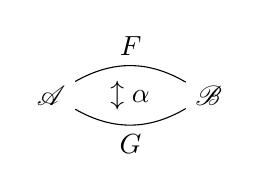
\begin{tikzpicture}
\node (CATA) at (-1,0) {$\CAT{A}$};
\node (CENTER) at (0,0) {$\updownarrow \alpha$};
\node (CATB) at (1,0) {$\CAT{B}$};
%\draw [<->] (Equity) -- (SelfEfficacy);
\path [-,bend left] (CATA) edge node [above] {$F$} (CATB);
\path [-,bend right] (CATA) edge node [below] {$G$} (CATB);
\end{tikzpicture}\\
Defining $\beta\circ\alpha$
\[
\begin{tikzcd}[row sep=huge]
    \CAT{A}
     \arrow[r, bend left=65, "F"{name=F}]
     \arrow[r, "G"{inner sep=0,fill=white,anchor=center,name=G}]
     \arrow[r, bend right=65, "H"{name=H, swap}]
     \arrow[from=F.south-|G,to=G,Rightarrow,shorten=2pt,"\alpha"] 
     \arrow[from=G,to=H.north-|G,Rightarrow,shorten=2pt,"\beta"] &
   \CAT{B}
\end{tikzcd} = 
\begin{tikzcd}[row sep=huge]
	\CAT{A}
     \arrow[r, bend left=35, "F"{name=F2}]
     \arrow[r, bend right=35, "H"{name=H2, swap}]
     \arrow[from=F2.south-|H2,to=H2,Rightarrow,shorten=2pt,"\beta\circ\alpha"] &
	\CAT{B}
\end{tikzcd}
\]
\end{center}



\subsection{Exercises}

\begin{enumerate}[label=1.3.\arabic*]
\setcounter{enumi}{24}
\item Find three examples of Natural Transformations not mentioned above.

\BLUE{\begin{enumerate}
	\item A group $G$ and its opposite $G^\OP$.  Both span the same set, but the left operations of $G$ are the right operations of $G^\OP$.  The function $F: G \to G\OP$ is the identity for the sets $F(A) = A$ along with the reverse homomorphism $F\circ f: G^\OP \to G$.  That is, where $f(gh)=f(g)f(h)$, $F(f)(gh)=F(f(h))F(f(g))$.
\end{enumerate}
}

\item Prove Lemma 1.3.11.

\item Let $\CAT{A}$ and $\CAT{B}$ be categories. Prove that $[\CAT{A}^\OP, \CAT{B}^\OP]\cong [\CAT{A},\CAT{B}]^\OP$

\item Let $A$ and $B$ be sets and denote $B^A$ the set of all functions from $A \to B$.  Write down:
\begin{enumerate}[label=(\alph*)]

\item A canonical function $A \times B^A \to B$.

\BLUE{Let $\phi: A \times B^A \to B$ then $\phi(a, f(a)) = f(a)$.
}

\item A canonical function $A \to B^{(B^A)}$.

(Although in principle there could be many such canonical function	, in both cases there is only one).

\BLUE{Let $\theta \in B^{(B^A)}$ which means $\theta: B^A \to B$.  Thus, $\theta(f(a)) \in B$ for some $f: A \to B$.  Let $\phi: A \to B^{(B^A)}$ then $\phi(a) = \theta(f(a))$ for some $\theta$ and some $f$, which must be in $B$.
}

\end{enumerate}

\item Here we consider natural transformations between functors whoe domain is a product of categories $\CAT{A}\times \CAT{B}$.  Your task is to show that naturality in two variables simultaneously is equivalent to naturality in each variable separately.

Take functors $F,G : \CAT{A}\times \CAT{B} \to \CAT{C}$.  For each $A\in \CAT{A}$, there are functors $F^A, G^A \: \CAT{B}\to \CAT{C}$, as in Exercise 1.2.25.  Similarly, for each $B \in \CAT{B}$, there are functors $F_B, G_B:\CAT{A}\to\CAT{C}$.

Let $(\alpha_{A,B}:F(A,B) \to G(A,B))_{A\in\CAT{A},B\in\CAT{B}}$ be a family of maps.  Show that this family is a natural transformation $F \to G$ if and only if it satisfies the following two conditions

\begin{itemize}
	\item for each $A \in \CAT{A}$, the family $(\alpha_{A,B}: F^A(B) \to G^A(B))_{B \in \CAT{B}}$ is a natural transformation $F^A \to G^A$;
	\item for each $B \in \CAT{B}$, the family $(\alpha_{A,B}:F_B(A)\to G_B(A))_{A\in \CAT{A}}$ is a natural transformation $F_B\to G_B$.
\end{itemize}

\item Let $G$ be a group.  For each $g \in G$, there is a unique homomorphism $\phi: \Z \to G$ satisfying $\phi(1)=g$.  Thus, elements of $G$ are essentially the same thing as homomorphisms $Z \to G$. When groups are regarded as one-object categories, homomorphisms $Z \to G$ are in turn the same a functors $\Z \to G$.  natural isomorphism defines an equivalence relation on the set of functors $\Z \to G$, and, therefore, an equivalence relation on $G$ itself.  What is this equivalence relation, in purely group-theoretic terms?

(First have a guess.  For a general group $G$, what equivalence relations on $G$ can you think  of?)

\item A \textbf{permutation} of a set $X$ is a bijection $X \to X$. Write $\CATSET{Sym}(X)$ for the set of permutations of $X$.  A \textbf{total order} on a set $X$ is an odrer $\le$ such that for all $x,y\in X$, either $x \le y$ or $ y\le x$; so a total order on a finite set amounts to a way of placing its elements in sequence.  Write $\CATSET{Ord}(X)$ for the set of total orders on $X$.

Let $\CAT{B}$ deonte the category of finite sets and bijections.

\begin{enumerate}
	\item Give a definition of $\CATSET{Sym}$ on maps in $\CAT{B}$ in such a way that $\CATSET{Sym}$ becomes a functor $\CAT{B}\to \CATSET{Set}$.  Do the same for $\CATSET{Ord}$.  Both your definitions should be canonical (no arbitrary choices).
	\item Show that there is no natural transformation $\CATSET{Sym}\to \CATSET{Ord}$.  (Hint: consider identity permutations.)
	\item For $n$-element set $X$, how many elements of the sets $\CATSET{Sym}(X)$ and $\CATSET{Ord}$ have?
\end{enumerate}
Conclude that $\CATSET{Sym}(X)\cong \CATSET{Ord}(X)$ for all $X \in \CAT{B}$, but not \textit{naturally} in $X \in \CAT{B}$.  (The moral is that each finite set $X$, there are exactly as many permutations of $X$ as there are total orders on $X$, but there is no natural way of matching them up.)

\item In this exercise, you will prove Proposition 1.3.18.  Let $F: \CAT{A} \to \CAT{B}$ be a functor.
\begin{enumerate}
	\item Suppose that $F$ is an equivalence.  Prove that $F$ is full, faithful and essentially surjective on objects.  (Hint: prove faithfulness before fullness.)
	\item Now suppose instead that $F$ is full, faithful and essentially surjective on objects.  For each $B \in \CAT{B}$, choose an object $G(B)$ of $\CAT{A}$ and an isomorphism $\epsilon_B:F(G(B)) \to B$.  Prove that $G$  extends to a functor in such a way that $(\epsilon_B)_{B \in \CAT{B}}$ is a natural isomorphism $FG \to 1_{\CAT{B}}$.  Then construct a natural isomorphism $1_{\CAT{A}} \to GF$, thus proving that $F$ is an equivalence.
\end{enumerate}

\item This exercise makes precise the idea that linear algebra can equivalently be done with matrices or with linear maps.

Fix a field $k$. Let $\CATSET{Mat}$ be the category whose objects are the natural numbers and with 
\begin{align*}
	\CATSET{Mat}(m,n)=\BRACKET{n\times m: \text{ matrices over }k}.
\end{align*}Prove that $\CATSET{Mat}$ is equivalent to $\CATSET{FDVect}$, the category of finite-dimensional vector spaces over $k$. does you equivalence involve \textit{a canonical} functor from $\CATSET{MAT}$ to $\CATSET{FDVect}$, or from $\CATSET{FDVect}$ to $\CATSET{Mat}$?

(Part of the exercise is to work out what composition in the cagtegory $\CATSET{Mat}$ is supposed to be; there is only on sensible possibility.  Propostition 1.3.18 makes the exercise easier.)

\item Show that equivalence of categories is an equivalence of relation.  (Not as obvious as it looks).
\end{enumerate}

\chapter{Adjoints}

\section{Definitions and Examples}

\begin{definition}[Bar Notation] 

Given an \DEFINE{adjunction} between $F$ and $G$ (i.e., a natural isomorphism) we define a \DEFINE{transpose} of morphism, that is, we call "$\bar{f}$ the transpose of $f$, and simlilarly for $g$, as in 
\begin{align*}
	\PAREN{F(A) \MORPHISM{g} B}&\mapsto \PAREN{A\MORPHISM{\bar{g}}G(B)},\\
	\PAREN{F(A)\MORPHISM{\bar{f}}B} &\leftarrow \PAREN{A \MORPHISM{f}G(B)}
\end{align*}i.e., $g:B \to B \implies \bar{g}: A \to A$

\end{definition}

\begin{definition}[The Naturality Axioms]

The \DEFINE{naturality axioms} have two parts.  Given an adjuction between $F$ and $G$, that is 
\begin{align*}
	\CAT{B}(F(A),B) &\cong \CAT{A}(A, G(B)) &(2.1)
\end{align*}that is being "naturally" isomorphic.  That is given $A \in \CAT{A}$ and $B\in \CAT{B}$ between maps $F(A) \to B$ and $G(B) \to A$ denoted by a horizontal bar in both directions:
\begin{align*}
	\CONJ{\PAREN{F(A)\MORPHISM{g}B\MORPHISM{q}B'}} &= \PAREN{A\MORPHISM{\bar{g}}G(B)\MORPHISM{G(q)}G(B')} & (2.2)
\end{align*}(that is, $\CONJ{q\circ g}=G(q)\circ \bar{g})$ for all $g$ and $q$, and 
\begin{align*}
	\CONJ{\PAREN{A'\MORPHISM{p}A\MORPHISM{f}G(B)}} &= \PAREN{F(A')\MORPHISM{F(p)}F(A)\MORPHISM{\bar{f}}B} & (2.3)
\end{align*}(that is, $\CONJ{f\circ p} = \bar{f}\circ F(p)$) for all $p$ and $f$.  It makes no difference whether we put the long bar over the left or the right of these equations, since bar is self-inverse.
\end{definition}
\HLINE
\begin{remark}Even though there is an adjuction between $F$ and $G$ (i.e., a natural isomorphism) the morphisms $f\in \CAT{A}$ implies $\bar{f}\in \CAT{B}$ and distinctly separate from $g \in \CAT{B}$ and $\bar{g}\in \CAT{A}$ and yet $\bar{\bar{f}}=f$.  That is, the bar operation relates $f$ through the isomorphism (2.1) (being 1-to-1 and onto) to its counterpart.
\end{remark}
\HLINE
\begin{remark}[From ChatGPT]

There exists an adjunction between $F : \CAT{C} \to \CAT{D}$ and $G:\CAT{D}\to \CAT{C}$ if
\begin{align*}
	\operatorname{Hom}_\CAT{D}(F(X), Y) \cong \operatorname{Hom}_\CAT{C}(X, G(Y))
\end{align*}for all $X \in \CAT{C}$ and $	Y \in \CAT{D}$.  That is, the set of all homomorphisms is isometric between the categories.\\
\\
Intuitively speaking:
\begin{enumerate}
	\item \textbf{Left Adjoint $F$: } ``Frees" up structure.
	\item \textbf{Right Adjoint $G$: } ``Forgets" or ``Extracts" structure.
\end{enumerate}

\end{remark}

\HLINE
\begin{remark}[ChatGPT] \textbf{Whats the difference between an "adjuction between $F$ and $G$" and "$G$ is the inverse of $F$"?}  
\begin{itemize}
	\item \textbf{Inverse:} $F \circ G = \operatorname{Id}_F$ and $G \circ F = \operatorname{Id}_G$.  
	
	\textbf{Meaning: }$F$ and $G$ define an \textbf{isomorphism of categories}. They are structure-preserving bijections at both the object and morphism levels.
	
	\item \textbf{Adjunction:} The \textit{natural isomorphism of Hom-sets} 
	\begin{align*}
		\operatorname{Hom}_\CAT{D}(F(X), Y) \cong \operatorname{Hom}_\CAT{C}(X, G(Y))
	\end{align*}This expresses a \textbf{universal property}.
	
	\textbf{That is: } $F$ is a left adjoint of $G$ if each $X\in \CAT{C}$ AND $Y \in \CAT{D}$ maps out of $F(X)$ correspond naturally to maps out of $X$ to $G(Y)$.
\end{itemize}
\end{remark}
\HLINE

\subsection{Exercises}

\begin{enumerate}[label=2.1.\arabic*]
\setcounter{enumi}{11}
\item  Find three examples of adjoint functors not mentioned above.  Do the same for intial and terminal objects.

\item What can be said about adjunctions between discrete categories?

\item Show that the naturality equation (2.2) and (2.3) can equivalently be replaced by the single equation 
\begin{align*}
	\CONJ{\PAREN{A'\MORPHISM{p}A\MORPHISM{f}G(B)\MORPHISM{G(q)}G(B')}} = \PAREN{F(A')\MORPHISM{F(p)}F(A)\MORPHISM{\bar{f}}B\MORPHISM{q}B'}
\end{align*}for all $p,f,$ and $q$.

\newcommand{\ADJOINT}[2]{\underset{\underset{#2}\longleftarrow}{\overset{\overset{#1}\longrightarrow}\bot }}


\item Show that the left adjoints preserve intitial objects: that is, $\CAT{A}\ADJOINT{F}{G}\CAT{B}$ and $I$ is the initial object of $\CAT{A}$, then $F(I)$ is the initial object of $\CAT{B}$.  Dually show that right adjoints preserve terminal objects.

\item Let $G$ be a group
\begin{enumerate}[label=(\alph*)]

	\item What interesting functors are there (in either direction) between $\CATSET{Set}$ and the category $[G,\CATSET{G}]$ for left $G$-sets?  Which of those functors are adjoint to which?
	
	\item Similarly, what interesting functors are there between $\CATSET{Vect}_k$ and category $[G,\CATSET{Vect}_k]$ of $k$-linear representations of $G$, and what adjunction are there between those functors?

\end{enumerate}

\item Fix a topological space $X$, and write $\CAT{O}(S)$ for the poset of open subsets of $X$, ordered by inclusion.  Let \begin{align*}
	\Delta:\CATSET{Set}\to \SQBRACKET{\CAT{O}(X)^\OP,\CATSET{Set}}
\end{align*}be the functor assigned to a set $A$ the presheaf $\Delta A$ with constant value $A$.  Exhibit a chain of adjoint functors
\begin{align*}
	\Lambda \dashv \Pi \dashv \Delta \dashv \Gamma \dashv \nabla.
\end{align*}

\section{adjunction via units and counits}

\end{enumerate}

\end{document}
